\documentclass[11pt]{beamer}
\usetheme{Dresden}
%\usecolortheme{beaver}
\usepackage[utf8]{inputenc}
\usepackage{amsmath}
\usepackage{amsfonts}
\usepackage{amssymb}
\usepackage{graphicx}
\usepackage{verbatim}
\usepackage{listings}
\usepackage{textcomp}
\usepackage{xcolor}
\author{Zheng Zheng}
\title{Topic 11 - Pipes, Filters and Regular Expressions }
%\setbeamercovered{transparent} 
%\setbeamertemplate{navigation symbols}{} 
%\logo{} 
\institute{McMaster University} 
\date{Winter 2023} 
\subject{COMPSCI 1XC3 - Computer Science Practice and Experience:
Development Basics} 
\stepcounter{section}

\definecolor{mGreen}{rgb}{0,0.6,0}
\definecolor{mGray}{rgb}{0.5,0.5,0.5}
\definecolor{mPurple}{rgb}{0.58,0,0.05}
\definecolor{mGreen2}{rgb}{0.05,0.65,0.05}
\definecolor{mGray2}{rgb}{0.55,0.55,0.55}
\definecolor{mPurple2}{rgb}{0.63,0.05,0.05}
\definecolor{backgroundColour}{rgb}{0.95,0.95,0.92}
\definecolor{backgroundColour2}{rgb}{0.95,0.92,0.95}

\lstdefinestyle{C}{
    backgroundcolor=\color{backgroundColour},   
    commentstyle=\color{mGreen},
    keywordstyle=\color{blue},
    numberstyle=\tiny\color{mGray},
    stringstyle=\color{mPurple},    
    basicstyle=\footnotesize,
    breakatwhitespace=false,         
    breaklines=true,                 
    captionpos=b,                    
    keepspaces=true,                 
    numbers=left,                    
    numbersep=5pt,                  
    showspaces=false,                
    showstringspaces=false,
    showtabs=false,                  
    tabsize=2,
    language=C
}

\definecolor{t_comment}{rgb}{0.2,1,0.2}
\definecolor{t_mGray}{rgb}{0.5,0.5,0.5}
\definecolor{t_mPurple}{rgb}{0.58,0,0.05}
\definecolor{t_blue}{rgb}{0.4,0.6,0.8}
\definecolor{t_mGreen2}{rgb}{0.05,0.65,0.05}
\definecolor{t_mGray2}{rgb}{0.75,0.75,0.75}
\definecolor{t_mPurple2}{rgb}{0.63,0.05,0.05}
\definecolor{t_bg}{rgb}{0.15,0.15,0.18}

\lstdefinestyle{terminal}{
    backgroundcolor=\color{t_bg},   
    commentstyle=\color{t_comment},
    keywordstyle=\color{t_blue},
    numberstyle=\tiny\color{t_mGray},
    stringstyle=\color{t_mGray2}, 
    basicstyle=\footnotesize\color{t_mGray2},
    breakatwhitespace=false,         
    breaklines=true,                 
    captionpos=b,                    
    keepspaces=true,                 
    numbers=none,                    
    numbersep=5pt,                  
    showspaces=false,                
    showstringspaces=false,
    showtabs=false,                  
    tabsize=2,
    language=bash
}

\definecolor{eggplant}{rgb}{0.52,0.11,0.3}

\usecolortheme[named=eggplant]{structure}

\begin{document}

\begin{frame}
\center
COMPSCI 1XC3 - Computer Science Practice and Experience:
Development Basics
\titlepage
% Toggle for C chapters
% Adapted from C: How to Program 8th ed., Deitel \& Deitel
\end{frame}

\begin{frame}
\tableofcontents
\end{frame}

\section[Pipes]{Stream Redirection}
\begin{frame}{Pipes of Different Types}
In Unix, we write programs to handle text streams because of the \emph{universality} of the interface.  
\begin{itemize}
\item We think about \texttt{stdin}, \texttt{stdout} and \texttt{stderr} as being \emph{streams of data}. 
\item How does one redirect a stream?  Using a \textbf{pipe} of course! 
\end{itemize}
\center
\begin{tabular}{| c | l |}
\hline 
Syntax & Description \\ \hline
\texttt{x $|$ y} & \texttt{x}'s \texttt{stdout} becomes  \texttt{y}'s \texttt{stdin}\\ \hline
\texttt{x $>$ y} & \texttt{x}'s \texttt{stdout} is written to file \texttt{y} \\ \hline
\texttt{x $<$ y} & file \texttt{y} is redirected to \texttt{x}'s \texttt{stdin} \\ \hline
\texttt{x 2$>$ y} & \texttt{x}'s \texttt{stderr} is written to file \texttt{y} \\ \hline 
\texttt{x \&$>$ y} & \texttt{x}'s \texttt{stdout} and \texttt{stderr} are written to file \texttt{y} \\ \hline 
\end{tabular}

\end{frame}

\begin{frame}[fragile=singleslide]{Check out These Pipes!}
We've used redirection to and from files a number of times in lab already, so let's take a look at $|$.
\begin{itemize}
\item Redirect long output so it can be scrolled through: 
\begin{lstlisting}[style=terminal]
$ make all | less
\end{lstlisting}
\item Retrieve the third line of a file
\begin{lstlisting}[style=terminal]
$ cat file | head -3 | tail -1
\end{lstlisting}
\item Sorted list of all unique file extensions in the current directory
\begin{lstlisting}[style=terminal]
$ ls | rev | cut -d'.' -f1 | rev | sort | uniq -c
\end{lstlisting}
\end{itemize}
\end{frame}

\begin{frame}[fragile=singleslide]{Piping and Loops}
You can even combine piping with loops in order to loop over the output of different commands, kind of like a Python for loop! 
\begin{lstlisting}[style=terminal]
ls | while read item
do
	echo "$item exists in this directory!"
done 
\end{lstlisting}
\end{frame}

\begin{frame}[fragile=singleslide]{Redirecting to Arguments with \texttt{xargs}}
When we pipe \texttt{stdout} to a command, the entire output is directed to \texttt{stdin}, regardless of separators (spaces, newlines, etc.). \\
\vspace{0.5em}
What if the command we want expects its input by argument, rather than by \texttt{stdin}?

\begin{lstlisting}[style=terminal]
$ ls | rm
	# tries to delete the entire output of ls
\end{lstlisting}

The \texttt{xargs} command will repeat other commands, feeding them input gathered from stdin.

\begin{lstlisting}[style=terminal]
$ ls | xargs rm
\end{lstlisting}
\begin{itemize}
\item In the above case, the output of \texttt{ls}, which is separated by whitespace, is broken up and fed to rm individually. 
\item This command therefore succeeds!
\end{itemize}
\end{frame}

\begin{frame}[fragile=singleslide]{Putting Arguments In! Their! Place!}
Let's say we want to copy all the files in a directory with the ``.txt'' extension into a directory named \texttt{tmp}.
\begin{lstlisting}[style=terminal]
$ find . -name *.txt | xargs cp /tmp
cp: -r not specified; omitting directory '/tmp'
\end{lstlisting}
\begin{itemize}
\item By default, xargs pipes in arguments at the \emph{end} of the list of arguments of the command its encapsulating.
\item In this case, cp is copying \emph{from} the place we want it to copy \emph{to}!
\end{itemize}
\begin{lstlisting}[style=terminal]
$ find . -name *.txt | xargs -I x cp x /tmp
\end{lstlisting}
\begin{itemize}
\item The \texttt{-I} flag lets us select where (and how many times) the argument will be inserted into the target command.  
\end{itemize}
\end{frame}

\section[Glob]{Glob Patterns}
\begin{frame}[fragile=singleslide]{Glob}
Glob patterns give us a way to represent filepaths that match a pattern.  We use special characters to represent multiple characters in various ways.
\begin{itemize}
\item \texttt{?} $\rightarrow$ Single character wildcard.  Character is required to exist.
\end{itemize}
\begin{lstlisting}[style=terminal]
$ rm Lab??/org.txt
\end{lstlisting}
\begin{itemize}
\item \texttt{\**} $\rightarrow$ zero or more continuous \texttt{?} wildcards.  Effectively, replaces any number of characters, including no characters at all!
\end{itemize}
\begin{lstlisting}[style=terminal]
$ rm *.c 
	# delete all .c files 
\end{lstlisting}
\begin{itemize}
\item $\{\}$ $\rightarrow$ choose between multiple specific strings (comma separated).
\end{itemize}
\begin{lstlisting}[style=terminal]
$ rm *.{c,o,h}
	# delete all .c, .o and .h files
\end{lstlisting}
\end{frame}

\begin{frame}[fragile=singleslide]{Glob (cont.)}
Brace expansion also supports sequences using \texttt{..} syntax.
\begin{lstlisting}[style=terminal]
$ echo {a..e}
a b c d e
$ echo {w..C}
W X Y Z [  ] ^ _ ` a b c
$ echo {10..-10}
10 9 8 7 6 5 4 3 2 1 0 -1 -2 -3 -4 -5 -6 -7 -8 -9 -10
\end{lstlisting}

It's generally a terrible idea to use glob characters literally in file and directory names, but if you \emph{really have to...}
\begin{itemize}
\item \textbackslash $\rightarrow$ Escape a special character.  
\end{itemize}
\begin{lstlisting}[style=terminal]
$ touch \*.c 
$ ls 
'*.rm'
\end{lstlisting}
\end{frame}

\begin{frame}[fragile=singleslide]{Glob (cont.)}
Glob patterns will expand to to a list of delimiter separated path names.
\begin{lstlisting}[style=terminal]
$ cp *.txt /tmp
	# Copies all files with a .txt extension to /tmp
$ cp file.txt ./*
	# Doesn't copy file.txt into all directories in the current director.
\end{lstlisting}
the second command above expands to:
\begin{lstlisting}[style=terminal]
$ cp file.tx ./dir1 ./dir2 ./dir3 ... ./dirX
\end{lstlisting}
This copies everything into \texttt{./dirX}!  
\end{frame}

\section[Find]{Searching For Files}
\begin{frame}[fragile=singleslide]{What a \texttt{find}!}
The \texttt{find} command allows us to locate files in our file system using glob patterns. 
\begin{lstlisting}[style=terminal]
$ find <starting directory> [-flags] -name <pattern>
\end{lstlisting}
\begin{itemize}
\item Unlike \texttt{cp} and \texttt{rm}, \texttt{find} automatically recurses through directories.  
\end{itemize}
\begin{lstlisting}[style=terminal]
$ find /bin -name ls
/bin/ls
\end{lstlisting}
\begin{itemize}
\item To limit how deep \texttt{find} goes to find matching files, use the \texttt{-maxdepth} flag.
\end{itemize}
\begin{lstlisting}[style=terminal]
$ find ~/ -maxdepth 5 -name *.c
# finds all .c files in the first five directory layers after $HOME
\end{lstlisting}
\end{frame}

\begin{frame}[fragile=singleslide]{\texttt{find}ers Keepers!}
\begin{itemize}
\item The \texttt{-f} flag tells \texttt{find} to target only files.
\item the \texttt{-d} flag tells \texttt{find} to target only directories.  
\item You can even use flags to invoke boolean operations, and perform multiple tests at once! 
\begin{lstlisting}[style=terminal]
$ find . -name *.c -or -name *.h
# finds all .c or .h files, starting in the current directory
$ find . -f -not -name *.py 
# finds all files which are not python source files, starting in the current directory
$ find -d -name Lab** -name *.tex
# finds all directories, starting in the current directory, matching both glob patterns.  
\end{lstlisting}
\end{itemize}
\end{frame}

\section[Regex]{Regular Expressions!}
% \begin{frame}
% \center
% 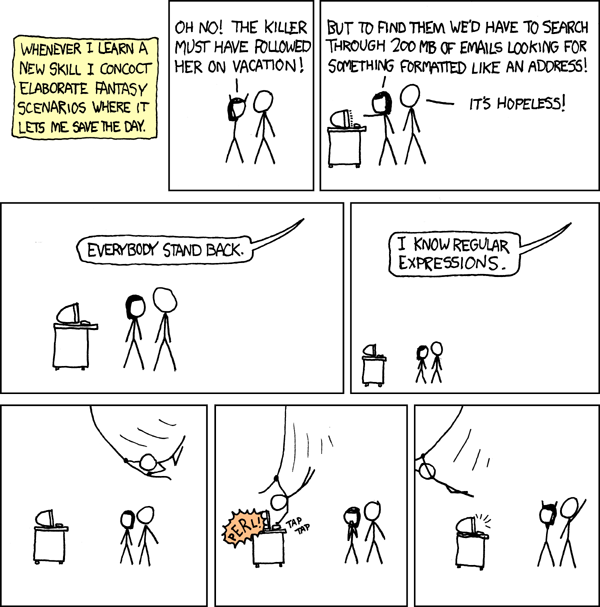
\includegraphics[scale=0.32]{regular_expressions.png}
% \end{frame}

\begin{frame}{Regular Expressions}
Glob patterns are wonderful for managing the file system, but lack the expressive power to be used on larger targets, such as files themselves.

\begin{itemize}
\item Enter the \textbf{Regular Expression} (or \textbf{regex})!
\item Based on a model of computaton called \textbf{Finite State Automata}, which is beyond the scope of this course.
\item Similarly to glob patterns, regular expressions allow us to write character patterns, which may then be used to test or search large groups of characters (i.e., files).
\item An excellent online tool for testing and debugging large and small regex is \url{https://regex101.com}
\end{itemize}
\end{frame}

\begin{frame}[fragile=singleslide]{Regex Syntax 1: Alternation}
\center
The vertical bar separates alternatives: \\
\texttt{a|b}
$$ \{a, b\} $$ 
\fbox{\includegraphics[scale=0.40]{regexOR.png}}
\end{frame}

\begin{frame}[fragile=singleslide]{Regex Syntax 2: Grouping}
\center 
Round braces determine how a regex operator is bound: \\
\texttt{Tom(ay|ah)to} 
$$\{Tomayto,Tomahto\}$$ 
\fbox{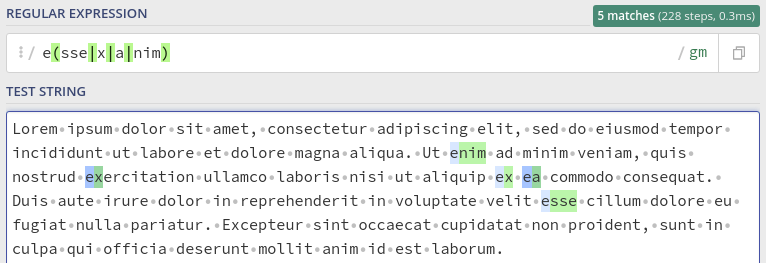
\includegraphics[scale=0.40]{regexBIND.png}}
\end{frame}

\begin{frame}[fragile=singleslide]{Regex Syntax 3: Quantification 1}
\center
A postfix plus specifies \emph{one or more} occurances of the character(s). 
\texttt{ab+c} \\
\vspace{0.5em}
$$ \{ abc, abbc, abbbc, ...\} $$ 
\fbox{\includegraphics[scale=0.4]{regexPLUS.png}}
\end{frame}

\begin{frame}{Regex Syntax 4 : Quantification 2}
\center
A postfix asterisk \texttt{\**} specifies \emph{zero or more} occurances. \\ 
\texttt{xy*z}
$$ \{ xz, xyz, xyyz, xyyyz, ... \} $$
\fbox{\includegraphics[scale=0.4]{regexTIMES.png}}
\end{frame}

\begin{frame}{Regex Syntax 5: Wildcards}
\center
The wildcard character \texttt{.} matches any character. \\
\texttt{a.b}
$$ {aac, abc, acc, adc, aec, ...} $$
\fbox{\includegraphics[scale=0.4]{regexWILD.png}}
\end{frame}

\section[Grep]{Advanced Searching}
\begin{frame}[fragile=singleslide]{The \texttt{grep}s of Wrath}
While \texttt{find} searches the \emph{names} of files, \texttt{grep} searches the \emph{contents} of files. 
\begin{lstlisting}[style=terminal]
$ grep <options> <pattern> <file(s)>
\end{lstlisting}
\begin{itemize}
\item As with many commands, we can specify multiple files to be searched using glob patterns, and we can search directories recursively using the \texttt{-r} flag.
\item If no file is specified, \texttt{grep} searches your working directory.  
\item The \texttt{-E} flag allows us to use \textbf{extended regular expressions}, which has some additional operators. 
\end{itemize}
\end{frame}

\begin{frame}[fragile=singleslide]{Grep Extended Regex Syntax 1} 
\begin{itemize}
\item \texttt{|} $\rightarrow$ works as expected.
\end{itemize}
\begin{lstlisting}[style=terminal]
$ grep -E 'It was the (best|worst) of times.' <file>
# Matches either 'It was the best of times' or 'It was the worst of times'
\end{lstlisting}
\begin{itemize}
\item \texttt{[]} $\rightarrow$ You can also use square braces to alternate many characters:
\end{itemize}

\begin{lstlisting}[style=terminal]
$ grep -E '[abcdefghijklmnopqrstuvwxyz]' <file>
# Matches any lowercase letter
\end{lstlisting}
\begin{itemize}
\item Notice how our regex is delimited by single quote characters! 
\item \texttt{.} is still the single character wildcard.
\end{itemize}
\begin{lstlisting}[style=terminal]
$ grep -E 'Super .ario' <file>
# Matches 'Super Aario', 'Super Bario', 'Super Cario', etc.
\end{lstlisting}
\end{frame}

\begin{frame}[fragile=singleslide]{Grep Extended Regex Syntax 2}
\begin{itemize}
\item \texttt{?} $\rightarrow$ postfix operator indicating an item is optional. 
\end{itemize}
\begin{lstlisting}[style=terminal]
$ grep -E 'a?b?c' <file>
# Matches 'c', 'ac', 'bc', and 'abc' 
\end{lstlisting}
\begin{itemize}
\item \texttt{*} $\rightarrow$ postfix operator indicating zero or more of an item 
\end{itemize}
\begin{lstlisting}[style=terminal]
$ grep -E 'too*' <file>
# Matches 'to', 'too', 'tooo', etc.
\end{lstlisting}
\begin{itemize}
\item \texttt{+} $\rightarrow$ postfix operator indicating one or more of an item.
\end{itemize}
\begin{lstlisting}[style=terminal]
$ grep -E 'Ba(na)+' <file>
# Matches 'Bana', 'Banana', 'Bananana', etc.
\end{lstlisting}
\begin{itemize}
\item As shown in the above example, round braces are still used for grouping. 
\end{itemize}
\end{frame}

\begin{frame}[fragile=singleslide]{Grep Extended Regex Syntax 3}
Although we have [ and ] to alternate larger groups of single characters, some common ones have been collected for us.
\vspace{0.5em}
\center 
\begin{tabular}{| c | l |}
\hline
Regex Code & Description \\ \hline
\texttt{[[:alnum:]]} & Alphanumerics \\ \hline
\texttt{[[:alpha:]]} & Alphabetics \\ \hline
\texttt{[[:blank:]]} & Spaces and tabs \\ \hline
\texttt{[[:space:]]} & All whitespace \\ \hline
\texttt{[[:digit:]]} & Numerics \\ \hline
\texttt{[[:lower:]]} & Lower-case alphabetics \\ \hline
\texttt{[[:upper:]]} & Upper-case alphabetics \\ \hline
\end{tabular}
\flushleft
\begin{lstlisting}[style=terminal]
$ grep -E '[[:lower:]]([[:upper:]][[:lower:]]+)*[[:blank:]]' <file>
# matchesAnyThingWrittenInCamelCase 
\end{lstlisting}
\end{frame}

\begin{frame}[fragile=singleslide]{Grep Extended Regex Syntax 4}
\begin{itemize}
\item Piping grep commands together find the \emph{union}.
\end{itemize}
\begin{lstlisting}[style=terminal]
$ grep 'pattern1' file | grep 'pattern2'
# Only matches lines containing both patterns
\end{lstlisting}
\begin{itemize}
\item \texttt{[\textasciicircum]} inverts the selection.
\end{itemize}
\begin{lstlisting}[style=terminal]
$ grep -E '[^(ordinary)]' <file>
# Matches anything but 'ordinary'
\end{lstlisting}
\begin{itemize}
\item \texttt{\textasciicircum} at the beginning of a pattern requires the pattern to start at the beginning of the line.
\item \texttt{\$} at the end of a pattern requires the pattern to end at the end of the line.
\end{itemize}
\begin{lstlisting}[style=terminal]
grep -E '^So anyways...$' <file>
# Matches 'So anyways...', but only if that's the entire line in the file.  
\end{lstlisting}
\end{frame}

\begin{frame}[fragile=singleslide]{That's What She \texttt{sed}!}
Any good programmer knows that find-and-replace is the most valuable tool any text editor can have.  \texttt{sed} (Stream EDitor) lets us perform find-and-replace operations with all the power of Bash and regular expressions!  
\begin{lstlisting}[style=terminal]
$ sed -i <flags> <pattern> <input>
# <pattern> := 's/<regex>/<string>/g' 
\end{lstlisting}
\begin{itemize}
\item The regular expression tells \texttt{sed} where to perform the substitutions.
\item The string is the replacement text. 
\end{itemize}
For example, the following operation:
\begin{lstlisting}[style=terminal]
$ sed -i 's/(oak|spruce|larch|ash|maple)/tree/g' file.txt
\end{lstlisting}
Replaces any of the above specified types of trees with the string ``tree''
\end{frame}

\begin{frame}[fragile=singleslide]{Under \texttt{sed}ation}
Of course, we can combine this with the power of \texttt{find} to be able to perform crazy operations like:
\begin{itemize}
\item Perform find and replace operations over every file in the filesystem (that we have permissions for)
\item Perform find and replace over all files in a directory and subdirectories of a particular file type.
\item Perform find and replace on a file we don't know the exact location of.
\begin{lstlisting}[style=terminal]
$ find ~/ --name *.c | sed -i 's/<stdio.h>/"stdio.h"/g' 
# replaces the braces on stdio.h with quotes in all .c files in the user's directory.  
\end{lstlisting}

\end{itemize}
\end{frame}

\section[Applications]{Various Applications}
\begin{frame}[fragile=singleslide]{Problems in Space}
In practice, searching commands can take a long time to execute, since they are often sifting through gigabytes of data (i.e., large portions of your filesystem)!
\begin{itemize}
\item If we have to perform a \texttt{grep} search with a large search area, but we know something about the files we need to search (like their all being .c files), we can pipe the result of \texttt{find} into \texttt{grep} to \emph{substantially} increase the speed of the search.  
\begin{lstlisting}[style=terminal]
$ find . -name *.tex | xargs grep -rai 'actually'
\end{lstlisting}
\item One problem we'll run into however, is that \texttt{xargs} considers 
\emph{both} newlines and space characters to be argument separators.  This can be a real problem if our directory names contain spaces! 
\end{itemize}  
\end{frame}

\begin{frame}[fragile=singleslide]{SPAAAAAAAAAAACE!!!!}
Fortunately, a number of commands (including find) allow us to set a special delimiter, which \texttt{xargs} can be configured to look for.
\begin{itemize}
\item Apply \texttt{-print0} to \texttt{find}
\item Apply \texttt{-0} to \texttt{xargs}
\item Profit!
\end{itemize}
\begin{lstlisting}[style=terminal]
$ find . -name *.tex -print0 | xargs -0 grep -rai 'actually'
./2MP3 Slides/Topic 11/Topic 11 - Other Topics in C++.tex:\item The four triangles that compose a tetrahedron require some constraints in order that they might actually form a tetrahedron.
...
\end{lstlisting}
\end{frame}

\section[Documentation]{Documentation}
\begin{frame}{Documentation!}
\center
\includegraphics[scale=0.15]{comments.png} \\
"The greatest obstacle to discovery is not ignorance -- it is the illusion of knowledge." -- Daniel Boorstin.
\end{frame}

\begin{frame}[fragile=singleslide]{Documentation!}
Some languages (like Haskell) are somewhat self-documenting.  C is not one of those languages.
\begin{itemize}
\item Code can be documented either:
\begin{itemize}
\item \emph{In the source code} $\rightarrow$ useful for programmers.
\item \emph{In an external document} $\rightarrow$ useful for all humans.  
\end{itemize}
\item A (recent?) trend in code documentation is \textbf{literate programming}.
\begin{itemize}
\item That is, the source code is annotated in such a way that some  documentation can be generated from it automatically.  
\end{itemize}
\end{itemize}
\end{frame}

\begin{frame}{Documentation Do's and Don'ts}
\begin{columns}
\begin{column}{0.5\textwidth}
\center
{\large \textbf{Do}}
\flushleft
\begin{itemize}
\item Write for your audience.
\begin{itemize}
\item i.e., other developers.
\end{itemize}
\item Use clear variable and function names (self-documentation)
\item Comment:
\begin{itemize}
\item The top of files
\item Functions
\item structs, typedefs
\item Control structures
\end{itemize}
\item Explain \emph{how} and \emph{why}
\end{itemize}
\end{column}
\begin{column}{0.5\textwidth}
\center
{\large \textbf{Don't}}
\flushleft
\begin{itemize}
\item Explain what each line of code does.
\item Explain how the language works.
\item Leave sarcastic comments. 
\item Be emotional in any way.
\item Comment each line. 
\item Write anything you wouldn't want anyone else to see (including your boss).
\end{itemize}
\end{column}
\end{columns}
\end{frame}

\begin{frame}{Types of Documentation}
\center
\includegraphics[scale=0.3]{documentation.png} \\
{\tiny Image forcibly collectivized from \href{https://blog.prototypr.io/software-documentation-types-and-best-practices-1726ca595c7f}{this source (link)}}
\end{frame}

\begin{frame}[fragile=singleslide]{Doxygen}
Wouldn't it be convenient to be able to generate documentation directly from your source code? 
\begin{itemize}
\item Enter Doxygen, a popular tool for documentation generation.
\item Available at \url{https://www.doxygen.nl/index.html}
\item Languages supported:
\end{itemize}
\begin{columns}
\begin{column}{0.25\textwidth}
\begin{itemize}
\item C
\item PHP
\item Fortran
\end{itemize}
\end{column}
\begin{column}{0.25\textwidth}
\begin{itemize}
\item C++
\item Java
\item VHDL
\end{itemize}
\end{column}
\begin{column}{0.25\textwidth}
\begin{itemize}
\item Objective-C
\item Python(!)
\item D
\end{itemize}
\end{column}
\begin{column}{0.25\textwidth}
\begin{itemize}
\item C\#
\item IDL
\end{itemize}
\vspace{1em}
\end{column}
\end{columns}
\vspace{0.25em}
\begin{itemize}
\item It can generate:
\end{itemize}
\vspace{-1em}
\begin{columns}
\begin{column}{0.25\textwidth}
\begin{itemize}
\item \LaTeX
\end{itemize}
\end{column}
\begin{column}{0.25\textwidth}
\begin{itemize}
\item HTML
\end{itemize}
\end{column}
\begin{column}{0.25\textwidth}
\begin{itemize}
\item man pages
\end{itemize}
\end{column}
\begin{column}{0.25\textwidth}
\begin{itemize}
\item others
\end{itemize}
\end{column}
\end{columns}
\end{frame}

\begin{frame}[fragile=singleslide]{Doxygen Tank}
To use Doxygen, you must first invoke:
\begin{lstlisting}[style=terminal]
$ doxygen -g
\end{lstlisting}
This generates ``Doxyfile'', a configuration file that has a \emph{large} number of configurable options.  
\begin{itemize}
\item Even more than Dwarf Fortress! 
\end{itemize}
It's important that the \texttt{PROJECT\_NAME} field be set, and if your source code is strewn among several directories that will also need to be configured.
\begin{itemize}
\item Doxygen checks your working directory for source code files by default.
\end{itemize}
To generate the document: 
\begin{lstlisting}[style=terminal]
$ doxygen Doxyfile
\end{lstlisting}
\end{frame}

\begin{frame}[fragile=singleslide]{Get her some Doxygen... Stat!}
To begin a doxygen comment in C, you have to \textbf{annotate} your source code.
\begin{lstlisting}[style=C]
/** <= Two asterisks start a "Doxygen comment".  This 
 * tags everything inside the comment for inclusion in 
 * the generated documentation.
 */
\end{lstlisting}
Position these at the top of functions, structs and typedefs to have Doxygen document said construct with your comment.  
\begin{itemize}
\item Doxygen also looks for \textbf{commands} to produce more informative documentation.
\item Commands start with the \texttt{@} character. 
\item \texttt{@param} documents function parameters.  
\item There are a bunch of these we'll be exploring in Lab 9.  
\end{itemize}
\end{frame}

\section[Acknowledge]{Acknowledge}
\begin{frame}{Acknowledge}
\center
\vspace{8em}
The contents of these slides were liberally borrowed (with permission) from slides from the Summer 2021 offering of 1XC3 (by Dr. Nicholas Moore).  
\end{frame}

% \section[Errata]{Errata}

% \begin{frame}{The Last Slide Comic}
% \center
% \includegraphics[scale=0.3]{comments2.jpg}
% \end{frame}

% \begin{frame}{Credits}
% \center
% \vspace{8em}
% A lot of the contents of these slides were liberally borrowed (with permission) from slides from the Winter 2020 offering of 1XA3 (by Curtis D'Alves), and the Winter 2021 offering of 1XC3 (by Dr. Kevin Browne).
% \end{frame}

\end{document}
